% Copyright 2004 by Till Tantau <tantau@users.sourceforge.net>.
%
% In principle, this file can be redistributed and/or modified under
% the terms of the GNU Public License, version 2.
%
% However, this file is supposed to be a template to be modified
% for your own needs. For this reason, if you use this file as a
% template and not specifically distribute it as part of a another
% package/program, I grant the extra permission to freely copy and
% modify this file as you see fit and even to delete this copyright
% notice. 

\documentclass[xcolor=table]{beamer}

\usepackage{graphicx}
\usepackage{subfig}
\usepackage{multirow}
% There are many different themes available for Beamer. A comprehensive
% list with examples is given here:
% http://deic.uab.es/~iblanes/beamer_gallery/index_by_theme.html
% You can uncomment the themes below if you would like to use a different
% one:
%\usetheme{AnnArbor}
%\usetheme{Antibes}
%\usetheme{Bergen}
%\usetheme{Berkeley}
%\usetheme{Berlin}
%\usetheme{Boadilla}
%\usetheme{boxes}
%\usetheme{CambridgeUS}
%\usetheme{Copenhagen}
%\usetheme{Darmstadt}
%\usetheme{default}
%\usetheme{Frankfurt}
%\usetheme{Goettingen}
%\usetheme{Hannover}
%\usetheme{Ilmenau}
%\usetheme{JuanLesPins}
%\usetheme{Luebeck}
\usetheme{Madrid}
%\usetheme{Malmoe}
%\usetheme{Marburg}
%\usetheme{Montpellier}
%\usetheme{PaloAlto}
%\usetheme{Pittsburgh}
%\usetheme{Rochester}
%\usetheme{Singapore}
%\usetheme{Szeged}
%\usetheme{Warsaw}


\title{Feasibility Study}

% A subtitle is optional and this may be deleted
\subtitle{Sparse Localization for Micro-UAVs in Disaster Response}

% - Give the names in the same order as the appear in the paper.
% - Use the \inst{?} command only if the authors have different
%   affiliation.

%\institute[University of Moratuwa] % (optional, but mostly needed)
% - Use the \inst command only if there are several affiliations.
% - Keep it simple, no one is interested in your street address.

\subject{Final Year Project}
% This is only inserted into the PDF information catalog. Can be left
% out. 
\date{}
% If you have a file called "university-logo-filename.xxx", where xxx
% is a graphic format that can be processed by latex or pdflatex,
% resp., then you can add a logo as follows:

% \pgfdeclareimage[height=0.5cm]{university-logo}{university-logo-filename}
% \logo{\pgfuseimage{university-logo}}

% Delete this, if you do not want the table of contents to pop up at
% the beginning of each subsection:

% Let's get started
\begin{document}
\begin{frame}
  \titlepage
  \begin{columns}
  \column{0.1\textwidth}
  \column{0.8\textwidth}
  	\begin{columns}
		\column{0.1\textwidth}
			\begin{center}
			
\includegraphics[scale=0.15]{UoM_Logo.png}
			\end{center}
		\column{0.9\textwidth}
			\begin{footnotesize}
			\begin{center}
			Department of Electronic and Telecommunication Engineering\\
			University of Moratuwa
			\end{center}
			\end{footnotesize}
	  \end{columns}
  \column{0.1\textwidth}
  \end{columns}
  
  \begin{center}
    \begin{tiny}
    \textbf{Collaboration} – Commonwealth Scientific and Industrial Research Organization, Australia
    \end{tiny}
  \end{center}  
\end{frame}

\begin{frame}{Team}
  \begin{itemize}
  \item Group Members
	\begin{itemize}
	\item 140083R - A.P.L.D.T.S. Chathuranga
	\item 140427D - D.K.M.A.M. Padmal
	\item 140076A - D.A. Bibile
	\item 140122M - N.U. Dharmasiri
	\end{itemize}
  \item Supervisors
	\begin{itemize}
	\item Dr. Peshala Jayasekara, University of Moratuwa
	\item Dr. Navinda Kottege, CSIRO, Australia (External Supervisor)
	\end{itemize}
  \end{itemize}
\end{frame}


\begin{frame}{Problem Statement}
  \begin{itemize}
  \item Disasters like building collapses have become a common occurrence
  \item Saving the lives of those who have been trapped is of utmost importance
  \end{itemize}
  \begin{figure}
  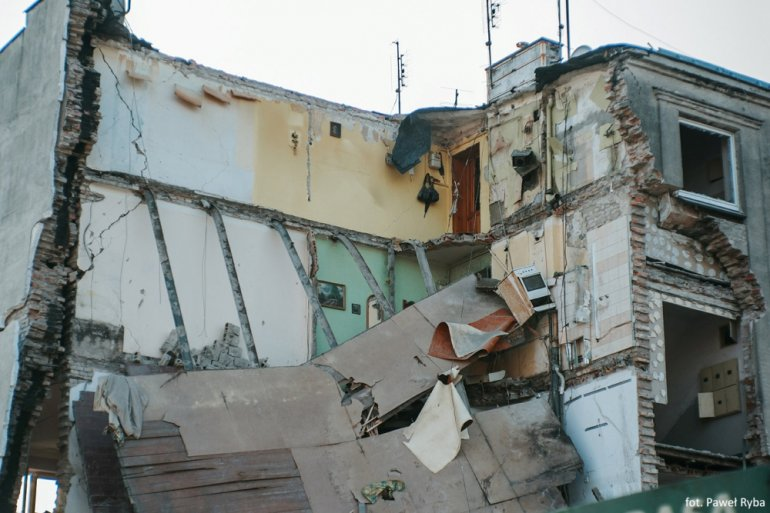
\includegraphics[scale=0.3]{Collapsed_Building.jpg}
  \end{figure}
\end{frame}

\begin{frame}{Problem Statement Contd.}
  \begin{itemize}
  \item However, it may risk the lives of those who are involved in rescue operations
  \item Also, usually there is a certain delay involved in conventional approaches
  \item There are limitations in using some of the newer methods as well
  	\begin{itemize}
  	\item Eg.: GPS localization is not possible inside buildings for autonomous robots
  	\end{itemize}
  \end{itemize}
\end{frame}

\begin{frame}{Proposed Solution}
  \begin{columns}
  \column{0.6\textwidth}
  \begin{itemize}
  \item To introduce a system which can help during rescue operations without risking further human lives
  \item These tasks are intended to be done using a micro UAV which has several advantages over other methods  
  \item Sparse sensing is to be used for localization because other conventional sensing techniques require a heavier payload. This leads to a shorter flight time, therefore reduces the effectiveness of the system
  \end{itemize}
  \column{0.4\textwidth}
  \begin{center}
  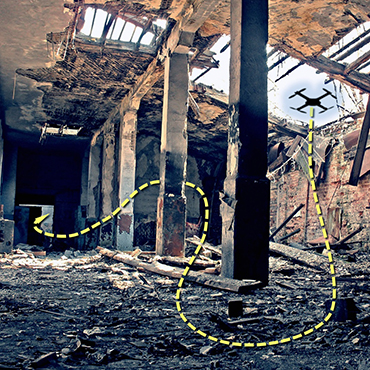
\includegraphics[scale=0.6]{Drone_Mobility.jpg}
  \end{center}
  \end{columns}
\end{frame}

\begin{frame}{Objectives}
  \begin{itemize}
  \item The autonomous vehicle should;
    \begin{itemize}
  	\item Enter and navigate through an unknown structure
  	\item Identify trapped people
  	\item Send their locations to the rescuers
  	\end{itemize}
  \item Simultaneous Localisation and Mapping (SLAM) using sparse sensing is the base of our approach
    \begin{itemize}
  	\item Localisation using sparse sensing is performed in order to navigate the UAV properly
  	\item A 3D sparse map should be created to help initiate the rescue operations
  	\end{itemize}
  \end{itemize}
\end{frame}

\begin{frame}{Scope}
  \begin{itemize}
  \item Use of an UAV that is small enough to enter into most parts of the collapsed structure
  \item The system only intends to provide sufficient information for the rescue teams to find trapped people. It would not be capable of mapping the structure with high precision
  \item Due to limited processing power available, structures that present highly complex scenarios are ignored
  \end{itemize}
\end{frame}

\begin{frame}{Evaluation of Alternative Strategies}{Building Collapse Rescue Methods}
  \begin{footnotesize}
  \begin{center}
  \setlength{\arrayrulewidth}{0.2mm}
  \setlength{\tabcolsep}{5pt}
  \renewcommand{\arraystretch}{1.2}
  \newcolumntype{s}{>{\columncolor[HTML]{b5e7a0}} p{2.4cm}}
  \arrayrulecolor[HTML]{000000}
 
  \begin{tabular}{ |p{3cm}|p{2.4cm}|p{2.4cm}|s|  }
  \hline
  &\multicolumn{3}{c|}{Method} \\
  \hline
  &\textbf{Human Rescue Teams}&\textbf{Heavy Machineries}&\textbf{Robots}\\
  \hline
  \textit{Preparation time} & High & High & Moderate \\
  \hline
 \textit{Danger to rescue teams} & High & High & Low \\
  \hline
  \textit{Time to identify trapped people} & Moderate & High & Moderate \\
  \hline
  \textit{Danger to trapped people} & Low & High & Low \\
  \hline
  \end{tabular}
  \end{center}
  \end{footnotesize}
\end{frame}

\begin{frame}{Evaluation of Alternative Strategies}{Robot Types}
  \begin{footnotesize}
  \begin{center}
  \setlength{\arrayrulewidth}{0.2mm}
  \setlength{\tabcolsep}{5pt}
  \renewcommand{\arraystretch}{1.2}
  \newcolumntype{s}{>{\columncolor[HTML]{b5e7a0}} p{3.55cm}}
  \arrayrulecolor[HTML]{000000}
 
  \begin{tabular}{ |p{3.55cm}|s|p{3.55cm}| }
  \hline
  \textbf{Tele-operated}&\textbf{Semi Autonomous}&\textbf{Fully Autonomous}\\
  \hline
  Trained operators required & Human in the loop method. & Can navigated automatically \\
  \hline
  Need to memorize the paths discovered by the robot. & Can automate the mapping process & Automatically maps the environment \\
  \hline
  Need time to perform precise maneuvers.  & Automated maneuvers & Automated maneuvers \\
  \hline
  Communication link is required. & Communication link is not mandatory. & Communication link is not mandatory \\
  \hline
  Human interaction in decision making & Human interaction in decision making & Automated decision making \\
  \hline
  \end{tabular}
  \end{center}
  \end{footnotesize}
\end{frame}

\begin{frame}{Evaluation of Alternative Strategies}{Robot Locomotion}
  \begin{footnotesize}
  \begin{center}
  \setlength{\arrayrulewidth}{0.2mm}
  \setlength{\tabcolsep}{5pt}
  \renewcommand{\arraystretch}{1.2}
  \newcolumntype{s}{>{\columncolor[HTML]{b5e7a0}} p{2cm}}
  \arrayrulecolor[HTML]{000000}
 
  \begin{tabular}{ |p{2cm}|p{2cm}|p{2cm}|s|p{2cm}| }
  \hline
  &\textbf{Ground Robots}&\textbf{Helicopter, Bicopter, Tricopter}&\textbf{Quadcopter}&\textbf{Pentacopters and above}\\
  \hline
  Speed & Low & High & High & High \\
  \hline
  Stability & High & Low & High & High \\
  \hline
  Mechanical complexity & Moderate & High & Low & Low \\
  \hline
  Ability to move to higher places & Low & High & High & High \\
  \hline
  High speed maneuvering & Not Possible & Not Possible & Possible & Possible \\
  \hline
  \end{tabular}
  \end{center}
  \end{footnotesize}
\end{frame}

\begin{frame}{Evaluation of Alternative Strategies}{Autonomous Quadcopter platforms}
  \begin{footnotesize}
  \begin{center}
  \setlength{\arrayrulewidth}{0.2mm}
  \setlength{\tabcolsep}{5pt}
  \renewcommand{\arraystretch}{1.2}
  \newcolumntype{s}{>{\columncolor[HTML]{b5e7a0}} p{2cm}}
  \arrayrulecolor[HTML]{000000}
 
  \begin{tabular}{ |p{2cm}|p{2cm}|p{2cm}|p{2cm}|s| }
  \hline
  &\textbf{DJI Phantom}\cite{DJIPhanthom}&\textbf{Pixhawk}\cite{Pixhawk}&\textbf{Parrot AR drone}\cite{Parrot}&\textbf{CrazyFlie}\cite{Crazyflie}\\
  \hline
  &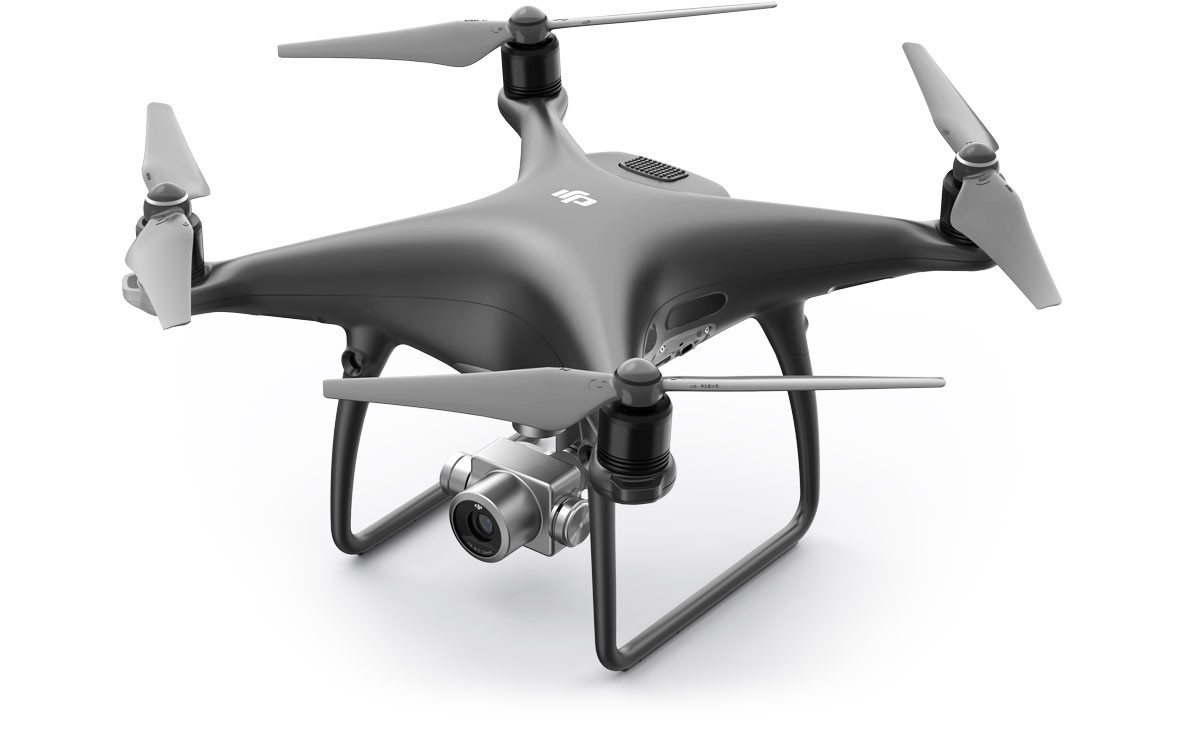
\includegraphics[scale=0.04]{DJI_Phanthom.jpg}&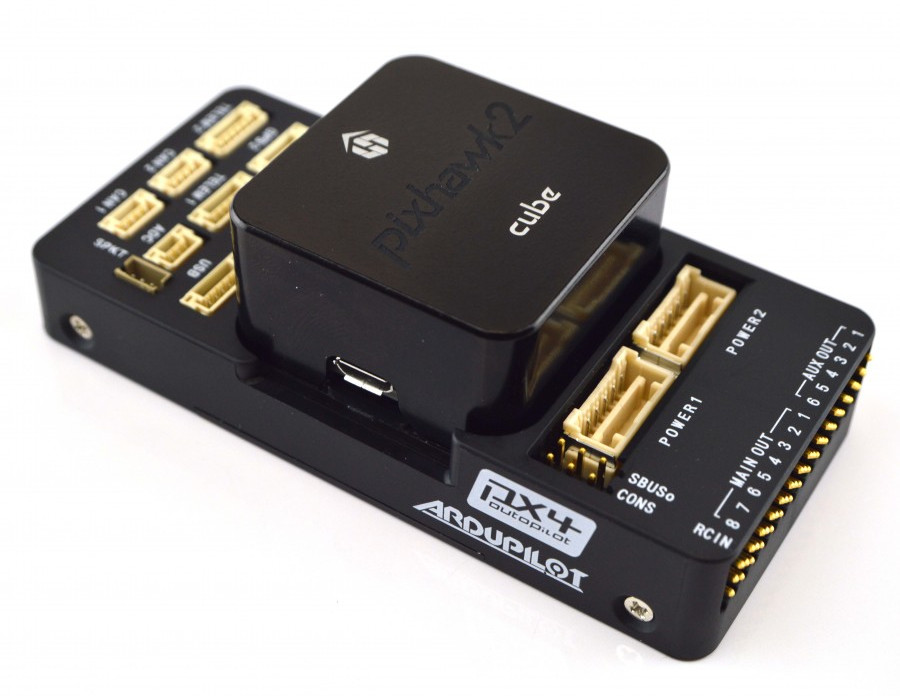
\includegraphics[scale=0.05]{Pixhawk.jpg}&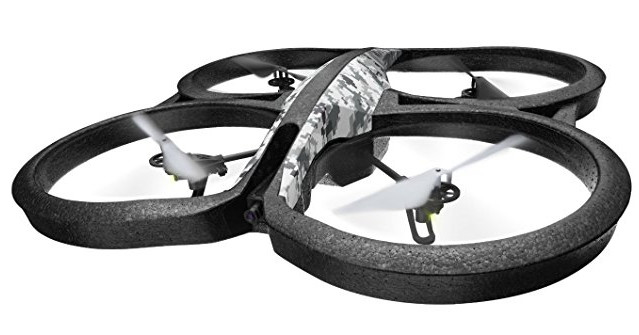
\includegraphics[scale=0.08]{Parrot.jpg}&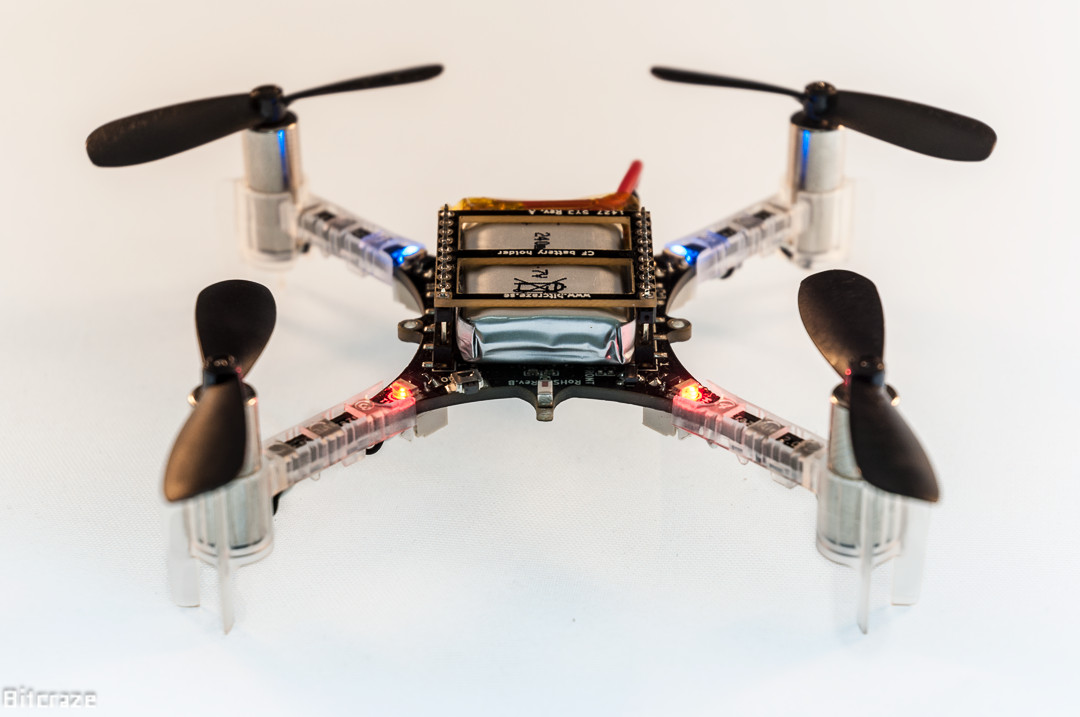
\includegraphics[scale=0.17]{Crazy_Flie_img.jpg}\\
  \hline
  Type & Complete system & Flight Controller only & Complete system & Complete system \\
  \hline
  Size & Medium & Vary & Medium & Very small \\
  \hline
  Access to hardware level & Not provided & Provided & Not provided & Provided \\
  \hline
  Electronic module integration & Not possible & Possible & Not possible & Possible \\
  \hline
  Cost & High & Medium & Medium & Low \\
  \hline
  \end{tabular}
  \end{center}
  \end{footnotesize}
  
  \begin{tiny}
  \begin{columns}
  \column{0.5\textwidth}
  [1]\texttt{www.dji.com/phantom-4/info}
  \column{0.5\textwidth}
  [3]\texttt{www.sciautonics.com/parrot-ar-drone-2-0-review}
  \end{columns}
  \begin{columns}
  \column{0.5\textwidth}
  [2]\texttt{ardupilot.org/copter/docs/common-pixhawk-overview}
  \column{0.5\textwidth}
  [4]\texttt{www.bitcraze.io/crazyflie-2/}
  \end{columns}
  \end{tiny}  
    
\end{frame}

\begin{frame}{Evaluation of Alternative Strategies}{Sensing methods for autonomous navigation and mapping}
  \begin{footnotesize}
  \begin{center}
  \setlength{\arrayrulewidth}{0.2mm}
  \setlength{\tabcolsep}{5pt}
  \renewcommand{\arraystretch}{1.2}
  \newcolumntype{s}{>{\columncolor[HTML]{b5e7a0}} p{3.55cm}}
  \arrayrulecolor[HTML]{000000}
 
  \begin{tabular}{ |p{3.55cm}|p{3.55cm}|s| }
  \hline
  \textbf{Vision based}&\textbf{LIDAR}&\textbf{Sparse Sensing}\\
  \hline
  [1][2]&[3][4]&[5][6] \\
  \hline
  3D map&3D point cloud&Low resolution grid maps \\
  \hline
  Extract features from images&Measure distance to objects&Measure distance to objects \\
  \hline
  \end{tabular}
  \end{center}
  \end{footnotesize}
  
  \begin{tiny}
  [1] C. Troiani, S. A. Zanati, and A. Martinelli, “A 3 points vision based approach for mav localization in gps denied environments,” in 2013 European Conference on Mobile Robots.
  
  [2] D. Li, Q. Li, L. Tang, S. Yang, N. Cheng, and J. Song, “Invariant observer-based state estimation for micro-aerial vehicles in gps-denied indoor environments using an rgb-d camera and mems inertial sensors”, Micromachines, vol. 6.
  
  [3] Lorenz Wellhausen, Renaud Dubé and  Abel Gawel, “Reliable real-time change detection and mapping for 3D LiDARs”, Safety, Security and Rescue Robotics (SSRR), 2017 IEEE International Symposium.
  
  [4] Paulo V. K. Borges and Alberto Elfes, “Real-time autonomous ground vehicle navigation in heterogeneous environments using a 3D LiDAR”, Intelligent Robots and Systems (IROS), 2017 IEEE/RSJ International Conference.

  [5] Kristopher R. Beevers and Wesley H. Huang “An Embedded Implementation of SLAM with Sparse Sensing”, Submitted the 2008 IEEE International Conference on Robotics \& Automation (ICRA 2008)
  
  [6] K. R. Beevers. “Mapping with limited sensing”. PhD thesis, Rensselaer Polytechnic Institute, Troy, NY, January 2007.
  \end{tiny}
  
\end{frame}

\begin{frame}{Evaluation of Alternative Strategies}{Sensing methods comparison}
  \begin{footnotesize}
  \begin{center}
  \setlength{\arrayrulewidth}{0.2mm}
  \setlength{\tabcolsep}{5pt}
  \renewcommand{\arraystretch}{1.2}
  \newcolumntype{s}{>{\columncolor[HTML]{b5e7a0}} p{2.4cm}}
  \arrayrulecolor[HTML]{000000}
 
  \begin{tabular}{ |p{3cm}|p{2.4cm}|p{2.4cm}|s|  }
  \hline
  &\multicolumn{3}{c|}{Method} \\
  \hline
  &\textbf{Vision based}&\textbf{High resolution range sensors}&\textbf{Distance measurement sensors}\\
  \hline
  \textit{Associated hardware} & Monocular/ Stereo Camera & LIDAR & \textbf{ToF} / IR / Sonar \\
  \hline
  \textit{Weight} & High & High & Very Low \\
  \hline
  \textit{Size} & Large & Large & Small \\
  \hline
  \textit{External lighting} & Required & Not required & Not required \\
  \hline
  \textit{Computational complexity} & High & High & Low \\
  \hline
  \textit{Power Consumption} & High & High & Low \\
  \hline
  \end{tabular}
  \end{center}
  \end{footnotesize}
\end{frame}

\begin{frame}{Project Architecture}
\begin{center}
  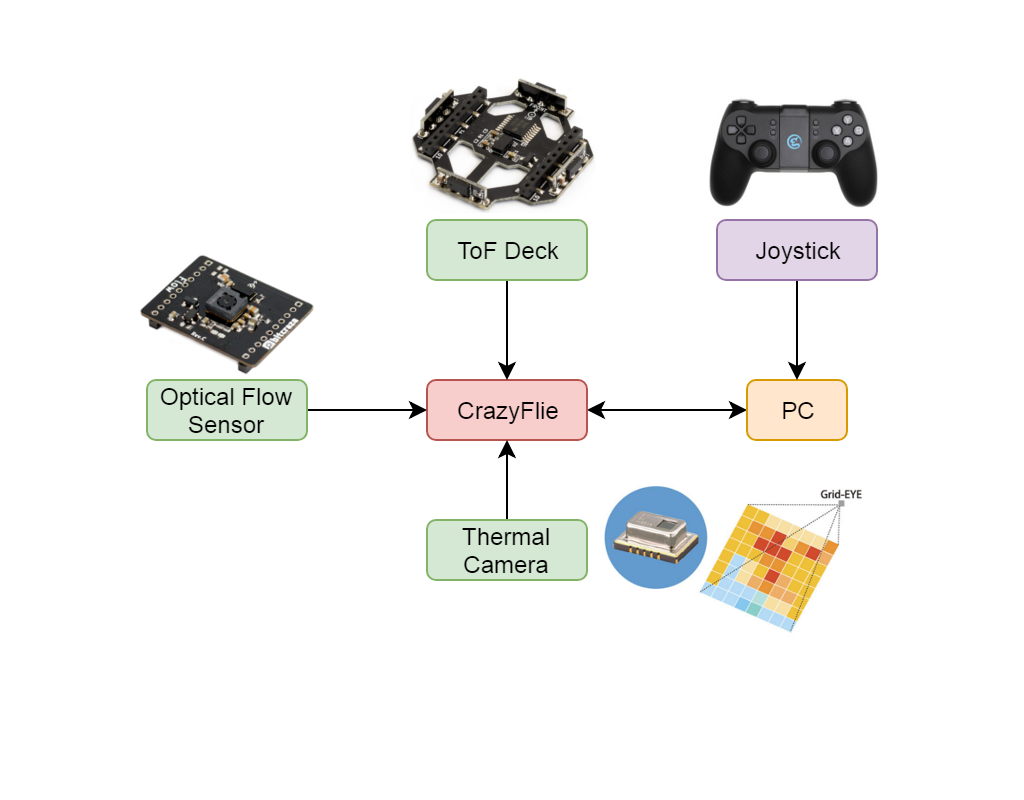
\includegraphics[scale=0.3]{FYP_Archi.png}
  \end{center}
\end{frame}

\begin{frame}{CrazyFlie 2.0 System Architecture}
  \begin{center}
  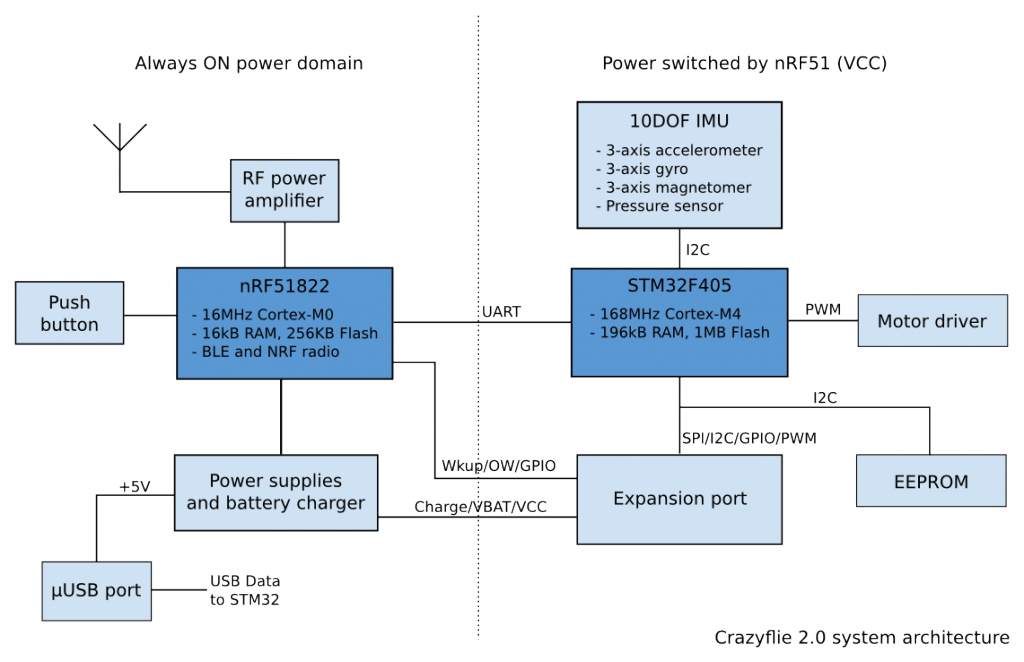
\includegraphics[scale=0.3]{Crazy_Archi.png}
  \end{center}
\end{frame}

\begin{frame}{Uniqueness of the Solution}
  \begin{itemize}
  \item Introduce indoor micro drones for disaster management in Sri Lanka
  \item Use sparse sensing to build low resolution 3D indoor maps
  \end{itemize}

  \begin{columns}
  \column{0.1\textwidth}
  \column{0.8\textwidth}
  \begin{block}{Potential Customers} 
  \begin{itemize}
  \item Ministry of Disaster Management
  \item National Disaster Management Council
  \item Fire and Rescue Services
  \end{itemize}
  \end{block}
  \column{0.1\textwidth}
  \end{columns} 
\end{frame}

\begin{frame}{Risk factors}
  \begin{footnotesize}
  \begin{center}
  \setlength{\arrayrulewidth}{0.2mm}
  \setlength{\tabcolsep}{5pt}
  \renewcommand{\arraystretch}{1.2}
  \newcolumntype{s}{>{\columncolor[HTML]{b5e7a0}} p{3.55cm}}
  \arrayrulecolor[HTML]{000000}
 
  \begin{tabular}{ |p{2cm}|p{3.55cm}|p{5cm}| }
  \hline
  \textbf{Category}&\textbf{Risk}&\textbf{Solution}\\
  \hline
  Technical&Limited battery life&Continuous battery level monitoring; Return to start position\\
  \hline
  Technical&Deprecated motors&Buy extra motors as backup\\
  \hline
  Technical&Damages to hardware&Use of software simulation to verify algorithms and using hardware at the final phase\\
  \hline
  Technical&Environmental impacts when testing on hardware&Design and build a customizable arena in university premises\\
  \hline
  Financial&Expenses for the hardware&Partially sponsored by CSIRO\\
  \hline
  \end{tabular}
  \end{center}
  \end{footnotesize}
\end{frame}

\begin{frame}{Resources}
  \begin{columns}
  \column{0.4\textwidth}
  \begin{itemize}
  \item Software Platforms
    \begin{itemize}
    \item ROS
    \item Gazebo
    \item MATLAB
    \item Python
    \item C++
    \end{itemize}
  \end{itemize}
  
  \begin{itemize}
  \item Hardware Platform
    \begin{itemize}
    \item CrazyFlie 2.0
    \end{itemize}
  \end{itemize}
  \column{0.6\textwidth}
  \begin{figure}
  
\includegraphics[scale=0.4]{Software_img.png}
  \end{figure}
  \begin{figure}
  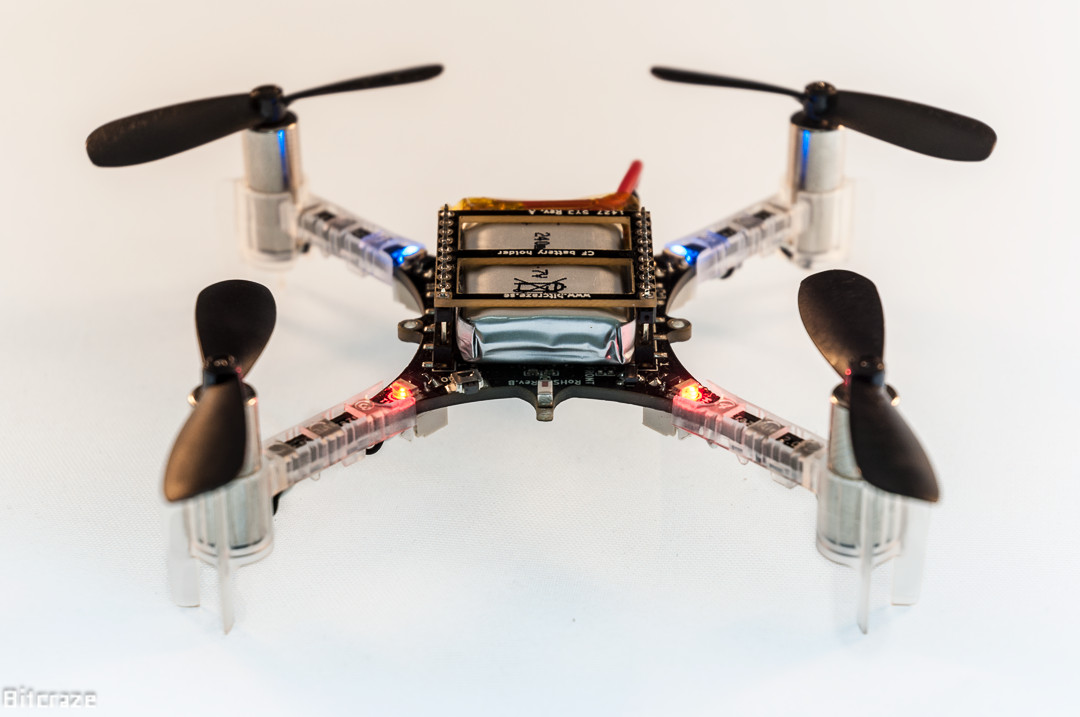
\includegraphics[scale=0.4]{Crazy_Flie_img.jpg}
  \end{figure}
  \end{columns}  
\end{frame}

\begin{frame}{Budget}
  \begin{footnotesize}
  \begin{center}
  \setlength{\arrayrulewidth}{0.2mm}
  \setlength{\tabcolsep}{5pt}
  \renewcommand{\arraystretch}{1.2}
  \newcolumntype{s}{>{\columncolor[HTML]{b5e7a0}} p{3.55cm}}
  \arrayrulecolor[HTML]{000000}
 
  \begin{tabular}{ |p{3.55cm}|p{3.55cm}|p{3.55cm}| }
  \hline
  \textbf{Component}&\textbf{Price}&\textbf{Status}\\
  \hline
  CrazyFlie 2.0 & USD 180.00 & Funded*\\
  \hline
  PMW3901 Optical flow sensor & USD 35.00 & Funded*\\
  \hline
  Radio receiver & USD 30.00 & Funded*\\
  \hline
  Range Sensor deck (Custom design) & USD 120.00 & Funded*\\
  \hline
  Micro FPV camera & USD 42.00 & Funded*\\
  \hline
  2.4GHz AV receiver & USD 68.00 & Funded*\\
  \hline
  AMG8833 Thermal camera & USD 40.00 & Not Funded\\
  \hline
  Extra motor pack & USD 20.00 & Not Funded\\
  \hline
  \end{tabular}
  \end{center}
  \end{footnotesize}
 \begin{flushright}
 {\small  *Funded by CSIRO, Australia.}
 \end{flushright}
\end{frame}

\begin{frame}{Task Delegation}

  \begin{columns}
  \column{0.1\textwidth}
  \column{0.8\textwidth}
  \begin{block}{Tharindu} 
  \begin{itemize}
  \item Building up the mathematical model
  \item Working on control systems
  \item Simulation on hardware platform
  \end{itemize}
  \end{block}
  
  \begin{block}{Padmal} 
  \begin{itemize}
  \item ROS related programming
  \item Algorithm implementation
  \item Simulation programming
  \end{itemize}
  \end{block}
  \column{0.1\textwidth}
  \end{columns} 
\end{frame}

\begin{frame}{Task Delegation Contd.}

  \begin{columns}
  \column{0.1\textwidth}
  \column{0.8\textwidth}
  \begin{block}{Dasun} 
  \begin{itemize}
  \item Setup on Hardware platform
  \item Simulation on hardware platform
  \item Simulation area management
  \end{itemize}
  \end{block}
  
  \begin{block}{Nadeera} 
  \begin{itemize}
  \item Building up the mathematical model
  \item ROS related programming
  \item Algorithm implementation
  \end{itemize}
  \end{block}
  \column{0.1\textwidth}
  \end{columns} 
\end{frame}

\begin{frame}{Project Timeline}
 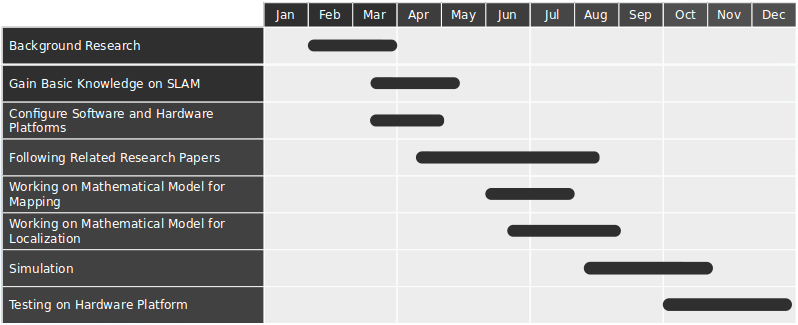
\includegraphics[width=12cm]{TimeLine.png}
\end{frame}

\begin{frame}{Sponsership}
 \begin{figure}
    \centering
    \subfloat{{
\includegraphics[width=3cm]{Data_61_img.jpg} }}
    \qquad
    \subfloat{{
\includegraphics[width=3cm]{CSIRO_Logo.png} }}
\end{figure}

\begin{center}
Robotics and Automation Laboratory,\\
Cyber Physical Systems,\\
Data 61,\\
Commonwealth Scientific and Industrial Research Organization,\\
Australia.
\end{center}
\end{frame}

\begin{frame}{Deliverables}
  \begin{enumerate}
  \item Autonomous navigation inside an unstructured environment
    \begin{enumerate}
    \item Obstacle avoidance
    \item Path planning
    \end{enumerate}
  \item A Low resolution 3D map of the environment
  \item Positions of the humans inside the environment. Expected to demonstrate using hot water bottles.
  \end{enumerate}
\end{frame}

\begin{frame}{Current Progress}
\begin{itemize}
\item Increase the stability of the quadcopter using the optical flow sensor
\item Build the radio link with the PC to send navigation commands
\item Test a state estimation algorithm including position tracking
\item Track the trajectory of the quadcopter while moving
\end{itemize}
% \begin{figure}
%    \centering
%    \subfloat{{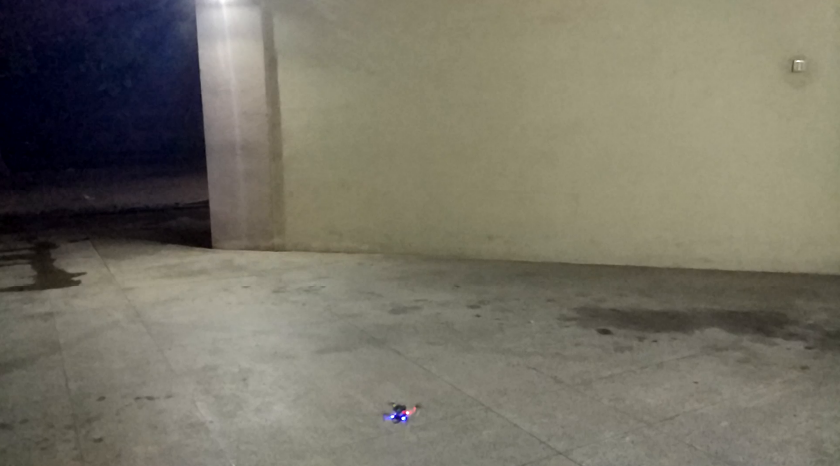
\includegraphics[width=5cm]{Video_img.png}}}
%    \qquad
%    \subfloat{{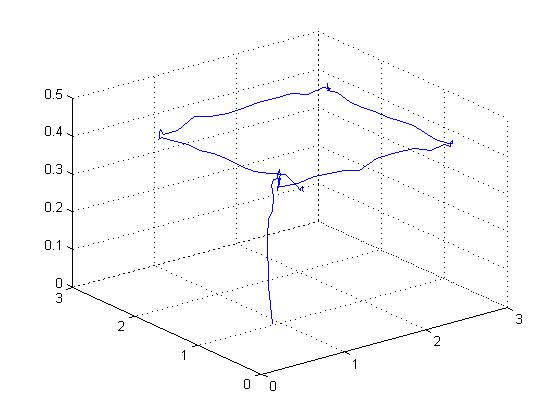
\includegraphics[width=5cm]{Trajectory_img.jpg} }}
%  \end{figure}
\end{frame}

\end{document}


